% !TEX root = ../pdf/lsr.tex
% [There are multiple lsr.tex files, but the one in ../pdf is the usual one]

%%%%%%%%%%%%%%%%%%%%%%
\chapter{Bayesian statistics \label{ch:bayes}}

\begin{quote}
{\it In our reasonings concerning matter of fact, there are all imaginable degrees of assurance, from the highest certainty to the lowest species of moral evidence. A wise man, therefore, proportions his belief to the evidence.} 

\hspace*{2cm} -- David Hume\FOOTNOTE{\url{http://en.wikiquote.org/wiki/David_Hume}.}
\end{quote}


%\begin{quote}
%{\it In God we trust; all others must bring data} \\
%\hspace*{2cm} -- William Edwards Deming (probably)\footnote{The preface to the Second Edition of the very excellent book ``The Elements of Statistical Learning'' \parencite{Hastie2009} mentions that ``on the Web, this quote has been widely attributed to both Deming and Robert W.
%Hayden; however Professor Hayden told us that he can claim no credit for this quote,
%and ironically we could find no ``data'' confirming that Deming actually said this.''}
%\end{quote}
%
%


%\begin{quote}
%{\it For many years, there has been controversy over `frequentist' versus `Bayesian' methods of inference, in which the writer has been an outspoken partisan on the Bayesian side. The record of this up to 1981 is given in an earlier book (Jaynes, 1983). In these old works there was a strong tendency, on both sides, to argue on the level of philosophy or ideology. We can now hold ourselves somewhat aloof from this because, thanks to recent work, there is no longer any need to appeal to such arguments. We are now in possession of proven theorems and masses of worked-out numerical examples. As a result, the superiority of Bayesian methods is now a thoroughly documented fact in a hundred different areas. One can argue with a philosophy; it is not so easy to argue with a computer printout.}\\
%\hspace*{2cm} -- E. T. Jaynes \parenciteyear{Jaynes2003}
%\end{quote}


\bigskip

The ideas I've presented to you in this book describe inferential statistics from the frequentist perspective. I'm not alone in doing this. In fact, almost every textbook given to undergraduate psychology students presents the opinions of the frequentist statistician as {\it the} theory of inferential statistics, the one true way to do things. I have taught this way for practical reasons. The frequentist view of statistics dominated the academic field of statistics for most of the 20th century, and this dominance is even more extreme among applied scientists. It was and is current practice among psychologists to use frequentist methods. Because frequentist methods are ubiquitous in scientific papers, every student of statistics needs to understand those methods, otherwise they will be unable to make sense of what those papers are saying! Unfortunately, in my opinion at least, the current practice in psychology is often misguided and the reliance on frequentist methods is partly to blame. In this chapter I explain why I think this and provide an introduction to Bayesian statistics, an approach that I think is generally superior to the orthodox approach.

This chapter comes in two parts. In Sections~\ref{sec:basicbayes} through \ref{sec:whybayes} I talk about what Bayesian statistics are all about, covering the basic mathematical rules for how it works as well as an explanation for why I think the Bayesian approach is so useful. Afterwards, I provide a brief overview of how you can do Bayesian versions of $t$-tests (Section~\ref{sec:ttestbf}).


\section{Probabilistic reasoning by rational agents\label{sec:basicbayes}}

From a Bayesian perspective statistical inference is all about {\it belief revision}. I start out with a set of candidate hypotheses $h$ about the world. I don't know which of these hypotheses is true, but do I have some beliefs about which hypotheses are plausible and which are not. When I observe the data, $d$, I have to revise those beliefs. If the data are consistent with a hypothesis, my belief in that hypothesis is strengthened. If the data are inconsistent with the hypothesis, my belief in that hypothesis is weakened. That's it! At the end of this section I'll give a precise description of how Bayesian reasoning works, but first I want to work through a simple example in order to introduce the key ideas. Consider the following reasoning problem.
\begin{quote}
{\it I'm carrying an umbrella. Do you think it will rain?}
\end{quote}
In this problem I have presented you with a single piece of data ($d =$ I'm carrying the umbrella), and I'm asking you to tell me your belief or hypothesis about whether it's raining. You have two alternatives, $h$: either it will rain today or it will not. How should you solve this problem? 

\SUBSECTION{Priors: what you believed before}

The first thing you need to do is ignore what I told you about the umbrella, and write down your pre-existing beliefs about rain. This is important. If you want to be honest about how your beliefs have been revised in the light of new evidence (data) then you {\it must} say something about what you believed before those data appeared! So, what might you believe about whether it will rain today? You probably know that I live in Australia and that much of Australia is hot and dry. The city of Adelaide where I live has a Mediterranean climate, very similar to southern California, southern Europe or northern Africa. I'm writing this in January and so you can assume it's the middle of summer. In fact, you might have decided to take a quick look on Wikipedia\FOOTNOTE{\url{http://en.wikipedia.org/wiki/Climate_of_Adelaide}} and discovered that Adelaide gets an average of 4.4 days of rain across the 31 days of January. Without knowing anything else, you might conclude that the probability of January rain in Adelaide is about 15\%, and the probability of a dry day is 85\%. If this is really what you believe about Adelaide rainfall (and now that I've told it to you I'm betting that this really {\it is} what you believe) then what I have written here is your \keyterm{prior distribution}, written $P(h)$:

\begin{center}
\begin{tabular}{c|c}
Hypothesis & Degree of Belief \\ \hline
Rainy day & 0.15 \\
Dry day & 0.85
\end{tabular}
\end{center}

\SUBSECTION{Likelihoods: theories about the data}

To solve the reasoning problem you need a theory about my behaviour. When does Dan carry an umbrella? You might guess that I'm not a complete idiot,\FOOTNOTE{It's a leap of faith, I know, but let's run with it okay?} and I try to carry umbrellas only on rainy days. On the other hand, you also know that I have young kids, and you wouldn't be all that surprised to know that I'm pretty forgetful about this sort of thing. Let's suppose that on rainy days I remember my umbrella about 30\% of the time (I really am awful at this). But let's say that on dry days I'm only about 5\% likely to be carrying an umbrella. So you might write out a little table like this:

\begin{center}
\begin{tabular}{c|cc}
 & \multicolumn{2}{|c}{Data} \\ 
Hypothesis & Umbrella & No umbrella \\ \hline
Rainy day & 0.30 & 0.70 \\
Dry day & 0.05 & 0.95 
\end{tabular}
\end{center}

\noindent
It's important to remember that each cell in this table describes your beliefs about what data $d$ will be observed, {\it given} the truth of a particular hypothesis $h$. This ``conditional probability'' is written $P(d|h)$, which you can read as ``the probability of $d$ given $h$''. In Bayesian statistics, this is referred to as the \keyterm{likelihood} of the data $d$ given the hypothesis $h$.\FOOTNOTE{Um. I hate to bring this up, but some statisticians would object to me using the word ``likelihood'' here. The problem is that the word ``likelihood'' has a very specific meaning in frequentist statistics, and it's not quite the same as what it means in Bayesian statistics. As far as I can tell Bayesians didn't originally have any agreed upon name for the likelihood, and so it became common practice for people to use the frequentist terminology. This wouldn't have been a problem except for the fact that the way that Bayesians use the word turns out to be quite different to the way frequentists do. This isn't the place for yet another lengthy history lesson but, to put it crudely, when a Bayesian says ``{\it a} likelihood function'' they're usually referring one of the {\it rows} of the table. When a frequentist says the same thing, they're referring to the same table, but to them ``{\it a} likelihood function'' almost always refers to one of the {\it columns}. This distinction matters in some contexts, but it's not important for our purposes.}

\SUBSECTION{The joint probability of data and hypothesis}

At this point all the elements are in place. Having written down the priors and the likelihood, you have all the information you need to do Bayesian reasoning. The question now becomes {\it how} do we use this information? As it turns out, there's a very simple equation that we can use here, but it's important that you understand why we use it so I'm going to try to build it up from more basic ideas.

Let's start out with one of the rules of probability theory. I listed it way back in Table~\ref{tab:probrules}, but I didn't make a big deal out of it at the time and you probably ignored it. The rule in question is the one that talks about the probability that {\it two} things are true. In our example, you might want to calculate the probability that today is rainy (i.e., hypothesis $h$ is true) \underline{and} I'm carrying an umbrella (i.e., data $d$ is observed). The \keyterm{joint probability} of the hypothesis and the data is written $P(d,h)$, and you can calculate it by multiplying the prior $P(h)$ by the likelihood $P(d|h)$. Mathematically, we say that
$$
P(d,h) = P(d|h) P(h)
$$
So, what is the probability that today is a rainy day {\it and} I remember to carry an umbrella? As we discussed earlier, the prior tells us that the probability of a rainy day is 15\%, and the likelihood tells us that the probability of me remembering my umbrella on a rainy day is 30\%. So the probability that both of these things are true is calculated by multiplying the two
\begin{eqnarray*}
P(\mbox{rainy}, \mbox{umbrella}) & = & P(\mbox{umbrella} | \mbox{rainy}) \times P(\mbox{rainy}) \\
& = & 0.30 \times 0.15 \\
& = & 0.045
\end{eqnarray*}
In other words, before being told anything about what actually happened, you think that there is a 4.5\% probability that today will be a rainy day and that I will remember an umbrella. However, there are of course {\it four} possible things that could happen, right? So let's repeat the exercise for all four. If we do that, we end up with the following table:
\begin{center}
\begin{tabular}{c|cc}
& Umbrella & No-umbrella \\ \hline
Rainy & 0.045 & 0.105 \\
Dry & 0.0425 & 0.8075
\end{tabular}
\end{center}
This table captures all the information about which of the four possibilities are likely. To really get the full picture, though, it helps to add the row totals and column totals. That gives us this table:
\begin{center}
\begin{tabular}{c|cc|c}
& Umbrella & No-umbrella & Total \\ \hline
Rainy & 0.0450 & 0.1050 & 0.15 \\
Dry & 0.0425 & 0.8075  & 0.85 \\ \hline
Total & 0.0875 & 0.9125 & 1
\end{tabular}
\end{center}
This is a very useful table, so it's worth taking a moment to think about what all these numbers are telling us. First, notice that the row sums aren't telling us anything new at all. For example, the first row tells us that if we ignore all this umbrella business, the chance that today will be a rainy day is 15\%. That's not surprising, of course, as that's our prior.\FOOTNOTE{Just to be clear, ``prior'' information is pre-existing knowledge or beliefs, before we collect or use any data to improve that information.} The important thing isn't the number itself. Rather, the important thing is that it gives us some confidence that our calculations are sensible! Now take a look at the column sums and notice that they tell us something that we haven't explicitly stated yet. In the same way that the row sums tell us the probability of rain, the column sums tell us the probability of me carrying an umbrella. Specifically, the first column tells us that on average (i.e., ignoring whether it's a rainy day or not) the probability of me carrying an umbrella is 8.75\%. Finally, notice that when we sum across all four logically-possible events, everything adds up to 1. In other words, what we have written down is a proper probability distribution defined over all possible combinations of data and hypothesis.

Now, because this table is so useful, I want to make sure you understand what all the elements correspond to and how they written:
\begin{center}
\begin{tabular}{r|rr|r}
& Umbrella & No-umbrella &  \\[6pt] \hline
Rainy & $P$(Umbrella, Rainy) & $P$(No-umbrella, Rainy) & $P$(Rainy) \\[6pt]
Dry & $P$(Umbrella, Dry) & $P$(No-umbrella, Dry)  & $P$(Dry) \\[6pt] \hline
 & $P$(Umbrella) & $P$(No-umbrella) & 
\end{tabular}
\end{center}
Finally, let's use ``proper'' statistical notation. In the rainy day problem, the data corresponds to the observation that I do or do not have an umbrella. So we'll let $d_1$ refer to the possibility that you observe me carrying an umbrella, and $d_2$ refers to you observing me not carrying one. Similarly, $h_1$ is your hypothesis that today is rainy, and $h_2$ is the hypothesis that it is not. Using this notation, the table looks like this:
\begin{center}
\begin{tabular}{r|rr|r}
& $d_1$ & $d_2$ &  \\[6pt] \hline
$h_1$ & $P(h_1, d_1)$ & $P(h_1, d_2)$ & $P(h_1)$ \\[6pt]
$h_2$ & $P(h_2, d_1)$ & $P(h_2, d_2)$ & $P(h_2)$ \\[6pt] \hline
 & $P(d_1)$ & $P(d_2)$ & 
\end{tabular}
\end{center}

\SUBSECTION{Updating beliefs using Bayes' rule}

The table we laid out in the last section is a very powerful tool for solving the rainy day problem, because it considers all four logical possibilities and states exactly how confident you are in each of them before being given any data. It's now time to consider what happens to our beliefs when we are actually given the data. In the rainy day problem, you are told that I really {\it am} carrying an umbrella. This is something of a surprising event. According to our table, the probability of me carrying an umbrella is only 8.75\%. But that makes sense, right? A guy carrying an umbrella on a summer day in a hot dry city is pretty unusual, and so you really weren't expecting that. Nevertheless, the data tells you that it is true. No matter how unlikely you thought it was, you must now adjust your beliefs to accommodate the fact that you now {\it know} that I have an umbrella.\FOOTNOTE{If we were being a bit more sophisticated, we could extend the example to accommodate the possibility that I'm lying about the umbrella. But let's keep things simple, shall we?} To reflect this new knowledge, our {\it revised} table must have the following numbers:
\begin{center}
\begin{tabular}{c|cc}
& Umbrella & No-umbrella  \\ \hline
Rainy &  & 0   \\
Dry &  & 0    \\ \hline
Total & 1 & 0 
\end{tabular}
\end{center}
In other words, the facts have eliminated any possibility of ``no umbrella'', so we have to put zeros into any cell in the table that implies that I'm not carrying an umbrella. Also, you know for a fact that I am carrying an umbrella, so the column sum on the left must be 1 to correctly describe the fact that $P(\mbox{umbrella})=1$.

What two numbers should we put in the empty cells? Again, let's not worry about the maths, and instead think about our intuitions. When we wrote out our table the first time, it turned out that those two cells had almost identical numbers, right? We worked out that the joint probability of ``rain and umbrella'' was 4.5\%, and the joint probability of ``dry and umbrella'' was 4.25\%. In other words, before I told you that I am in fact carrying an umbrella, you'd have said that these two events were almost identical in probability, yes? But notice that {\it both} of these possibilities are consistent with the fact that I actually am carrying an umbrella. From the perspective of these two possibilities, very little has changed. I hope you'd agree that it's {\it still} true that these two possibilities are equally plausible. So what we expect to see in our final table is some numbers that preserve the fact that ``rain and umbrella'' is {\it slightly} more plausible than ``dry and umbrella'', while still ensuring that numbers in the table add up. Something like this, perhaps?
\begin{center}
\begin{tabular}{c|cc}
& Umbrella & No-umbrella  \\ \hline
Rainy & 0.514 & 0   \\
Dry & 0.486 & 0    \\ \hline
Total & 1 & 0 
\end{tabular}
\end{center}
What this table is telling you is that, after being told that I'm carrying an umbrella, you believe that there's a 51.4\% chance that today will be a rainy day, and a 48.6\% chance that it won't. That's the answer to our problem! The \keyterm{posterior probability} of rain $P(h|d)$ given that I am carrying an umbrella is 51.4\%

How did I calculate these numbers? You can probably guess. To work out that there was a 0.514 probability of ``rain'', all I did was take the 0.045 probability of ``rain and umbrella'' and divide it by the 0.0875 chance of ``umbrella''. This produces a table that satisfies our need to have everything sum to 1, and our need not to interfere with the relative plausibility of the two events that are actually consistent with the data. To say the same thing using fancy statistical jargon, what I've done here is divide the joint probability of the hypothesis and the data $P(d,h)$ by the \keyterm{marginal probability} of the data $P(d)$, and this is what gives us the posterior probability of the hypothesis {\it given} the data that have been observed. To write this as an equation \FOOTNOTE{You might notice that this equation is actually a restatement of the same basic rule I listed at the start of the last section. If you multiply both sides of the equation by $P(d)$, then you get $P(d) P(h| d) = P(d,h)$, which is the rule for how joint probabilities are calculated. So I'm not actually introducing any ``new'' rules here, I'm just using the same rule in a different way.}
$$
P(h | d) = \frac{P(d,h)}{P(d)}
$$
However, remember what I said at the start of the last section, namely that the joint probability $P(d,h)$ is calculated by multiplying the prior $P(h)$ by the likelihood $P(d|h)$. In real life, the things we actually know how to write down are the priors and the likelihood, so let's substitute those back into the equation. This gives us the following formula for the posterior probability
$$
P(h | d) = \frac{P(d|h) P(h)}{P(d)}
$$
And this formula, folks, is known as \keyterm{Bayes' rule}. It describes how a learner starts out with prior beliefs about the plausibility of different hypotheses, and tells you how those beliefs should be revised in the face of data. In the Bayesian paradigm, all statistical inference flows from this one simple rule.


\section{Bayesian hypothesis tests~\label{sec:bayesianhypothesistests}}

In Chapter~\ref{ch:hypothesistesting} I described the orthodox approach to hypothesis testing. It took an entire chapter to describe, because null hypothesis testing is a very elaborate contraption that people find very hard to make sense of. In contrast, the Bayesian approach to hypothesis testing is incredibly simple. Let's pick a setting that is closely analogous to the orthodox scenario. There are two hypotheses that we want to compare, a null hypothesis $h_0$ and an alternative hypothesis $h_1$. Prior to running the experiment we have some beliefs $P(h)$ about which hypotheses are true. We run an experiment and obtain data $d$. Unlike frequentist statistics, Bayesian statistics does allow us to talk about the probability that the null hypothesis is true. Better yet, it allows us to calculate the \keyterm{posterior probability of the null hypothesis}, using Bayes' rule
$$
P(h_0 | d) = \frac{P(d|h_0) P(h_0)}{P(d)}
$$
This formula tells us exactly how much belief we should have in the null hypothesis after having observed the data $d$. Similarly, we can work out how much belief to place in the alternative hypothesis using essentially the same equation. All we do is change the subscript
$$
P(h_1 | d) = \frac{P(d|h_1) P(h_1)}{P(d)}
$$
It's all so simple that I feel like an idiot even bothering to write these equations down, since all I'm doing is copying Bayes rule from the previous section.\FOOTNOTE{Obviously, this is a highly simplified story. All the complexity of real life Bayesian hypothesis testing comes down to how you calculate the likelihood $P(d|h)$ when the hypothesis $h$ is a complex and vague thing. I'm not going to talk about those complexities in this book, but I do want to highlight that although this simple story is true as far as it goes, real life is messier than I'm able to cover in an introductory stats textbook.}

\subsection{The Bayes factor}

In practice, most Bayesian data analysts tend not to talk in terms of the raw posterior probabilities $P(h_0|d)$ and $P(h_1|d)$. Instead, we tend to talk in terms of the \keyterm{posterior odds} ratio. Think of it like betting. Suppose, for instance, the posterior probability of the null hypothesis is 25\%, and the posterior probability of the alternative is 75\%. The alternative hypothesis is three times as probable as the null, so we say that the {\it odds} are 3:1 in favour of the alternative. Mathematically, all we have to do to calculate the posterior odds is divide one posterior probability by the other
$$
\frac{P(h_1 | d)}{P(h_0 | d)} = \frac{0.75}{0.25} = 3
$$
Or, to write the same thing in terms of the equations above
$$
\frac{P(h_1 | d)}{P(h_0 | d)} = \frac{P(d|h_1)}{P(d|h_0)} \times \frac{P(h_1)}{P(h_0)}
$$

Actually, this equation is worth expanding on. There are three different terms here that you should know. On the left hand side, we have the posterior odds, which tells you what you believe about the relative plausibilty of the null hypothesis and the alternative hypothesis {\it after} seeing the data. On the right hand side, we have the \keyterm{prior odds}, which indicates what you thought {\it before} seeing the data. In the middle, we have the \keyterm{Bayes factor}, which describes the amount of evidence provided by the data
$$
\begin{array}{ccccc}\displaystyle
\frac{P(h_1 | d)}{P(h_0 | d)} &=& \displaystyle\frac{P(d|h_1)}{P(d|h_0)} &\times& \displaystyle\frac{P(h_1)}{P(h_0)} \\[6pt] \\[-2pt]
\uparrow && \uparrow && \uparrow \\[6pt]
\mbox{Posterior odds} && \mbox{\keyterm{Bayes factor}} && \mbox{Prior odds}
\end{array}
$$
The Bayes factor (sometimes abbreviated as \keyterm{BF}) has a special place in Bayesian hypothesis testing, because it serves a similar role to the $p$-value in orthodox hypothesis testing. The Bayes factor quantifies the strength of evidence provided by the data, and as such it is the Bayes factor that people tend to report when running a Bayesian hypothesis test. The reason for reporting Bayes factors rather than posterior odds is that different researchers will have different priors. Some people might have a strong bias to believe the null hypothesis is true, others might have a strong bias to believe it is false. Because of this, the polite thing for an applied researcher to do is report the Bayes factor. That way, anyone reading the paper can multiply the Bayes factor by their own {\it personal} prior odds, and they can work out for themselves what the posterior odds would be. In any case, by convention we like to pretend that we give equal consideration to both the null hypothesis and the alternative, in which case the prior odds equals 1, and the posterior odds becomes the same as the Bayes factor.

\subsection{Interpreting Bayes factors}

One of the really nice things about the Bayes factor is the numbers are inherently meaningful. If you run an experiment and you compute a Bayes factor of 4, it means that the evidence provided by your data corresponds to betting odds of 4:1 in favour of the alternative. However, there have been some attempts to quantify the standards of evidence that would be considered meaningful in a scientific context. The two most widely used are from \textcite{Jeffreys1961} and \textcite{Kass1995}. Of the two, I tend to prefer the \textcite{Kass1995} table because it's a bit more conservative. So here it is:
\begin{center}
\begin{tabular}{r|r}
Bayes factor & Interpretation \\ \hline
1 - 3 & Negligible evidence \\
3 - 20 & Positive evidence \\
20 - 150 & Strong evidence \\
$>$150 & Very strong evidence
\end{tabular}
\end{center} 
And to be perfectly honest, I think that even the \textcite{Kass1995} standards are being a bit charitable. If it were up to me, I'd have called the ``positive evidence'' category ``weak evidence''. To me, anything in the range 3:1 to 20:1 is ``weak'' or ``modest'' evidence at best. But there are no hard and fast rules here. What counts as strong or weak evidence depends entirely on how conservative you are and upon the standards that your community insists upon before it is willing to label a finding as ``true''. 

In any case, note that all the numbers listed above make sense if the Bayes factor is greater than 1 (i.e., the evidence favours the alternative hypothesis). However, one big practical advantage of the Bayesian approach relative to the orthodox approach is that it also allows you to quantify evidence {\it for} the null. When that happens, the Bayes factor will be less than 1. You can choose to report a Bayes factor less than 1, but to be honest I find it confusing. For example, suppose that the likelihood of the data under the null hypothesis $P(d|h_0)$ is equal to 0.2, and the corresponding likelihood $P(d|h_1)$ under the alternative hypothesis is 0.1. Using the equations given above,  Bayes factor here would be
$$ 
\mbox{BF} = \frac{P(d|h_1)}{P(d|h_0)} = \frac{0.1}{0.2} = 0.5
$$
Read literally, this result tells is that the evidence in favour of the alternative is 0.5 to 1. I find this hard to understand. To me, it makes  a lot more sense to turn the equation ``upside down'', and report the amount op evidence in favour of the {\it null}. In other words, what we calculate is this
$$ 
\mbox{BF}^\prime = \frac{P(d|h_0)}{P(d|h_1)} = \frac{0.2}{0.1} = 2
$$
And what we would report is a Bayes factor of 2:1 in favour of the null. Much easier to understand, and you can interpret this using the table above. 


\section{Why be a Bayesian?\label{sec:whybayes}}

Up to this point I've focused exclusively on the logic underpinning Bayesian statistics. We've talked about the idea of ``probability as a degree of belief'', and what it implies about how a rational agent should reason about the world. The question that you have to answer for yourself is this: how do {\it you} want to do your statistics? Do you want to be an orthodox statistician, relying on sampling distributions and $p$-values to guide your decisions? Or do you want to be a Bayesian, relying on things like prior beliefs, Bayes factors and the rules for rational belief revision? And to be perfectly honest, I can't answer this question for you. Ultimately it depends on what you think is right. It's your call and your call alone. That being said, I can talk a little about why {\it I} prefer the Bayesian approach. 

\subsection{Statistics that mean what you think they mean}

\begin{quote}
{\it You keep using that word. I do not think it means what you think it means} 

\hspace*{2cm} -- Inigo Montoya, The Princess Bride\FOOTNOTE{\url{http://www.imdb.com/title/tt0093779/quotes}. I should note in passing that I'm not the first person to use this quote to complain about frequentist methods. Rich Morey and colleagues had the idea first. I'm shamelessly stealing it because it's such an awesome pull quote to use in this context and I refuse to miss any opportunity to quote {\it The Princess Bride}.}
\end{quote}

To me, one of the biggest advantages to the Bayesian approach is that it answers the right questions. Within the Bayesian framework, it is perfectly sensible and allowable to refer to ``the probability that a hypothesis is true''. You can even try to calculate this probability. Ultimately, isn't that what you {\it want} your statistical tests to tell you? To an actual human being, this would seem to be the whole {\it point} of doing statistics, i.e., to determine what is true and what isn't. Any time that you aren't exactly sure about what the truth is, you should use the language of probability theory to say things like ``there is an 80\% chance that Theory A is true, but a 20\% chance that Theory B is true instead''. 

This seems so obvious to a human, yet it is explicitly forbidden within the orthodox framework. To a frequentist, such statements are a nonsense because ``the theory is true'' is not a repeatable event. A theory is true or it is not, and no probabilistic statements are allowed, no matter how much you might want to make them. There's a reason why, back in Section~\ref{sec:pvalue}, I repeatedly warned you {\it not} to interpret the $p$-value as the probability that the null hypothesis is true. There's a reason why almost every textbook on statstics is forced to repeat that warning. It's because people desperately {\it want} that to be the correct interpretation. Frequentist dogma notwithstanding, a lifetime of experience of teaching undergraduates and of doing data analysis on a daily basis suggests to me that most actual humans think that ``the probability that the hypothesis is true'' is not only meaningful, it's the thing we care {\it most} about. It's such an appealing idea that even trained statisticians fall prey to the mistake of trying to interpret a $p$-value this way. For example, here is a quote from an official Newspoll report in 2013, explaining how to interpret their (frequentist) data analysis:\FOOTNOTE{\url{http://about.abc.net.au/reports-publications/appreciation-survey-summary-report-2013/}}
\begin{quote}
Throughout the report, where relevant, statistically significant changes have been noted. All significance tests have been based on the 95 percent level of confidence. {\bf This means that if a change is noted as being statistically significant, there is a 95 percent probability that a real change has occurred}, and is not simply due to chance variation. (emphasis added)
\end{quote}
Nope! That's {\it not} what $p<.05$ means. That's {\it not} what 95\% confidence means to a frequentist statistician. The bolded section is just plain wrong. Orthodox methods cannot tell you that ``there is a 95\% chance that a real change has occurred'', because this is not the kind of event to which frequentist probabilities may be assigned. To an ideological frequentist, this sentence should be meaningless. Even if you're a more pragmatic frequentist, it's still the wrong definition of a $p$-value. It is simply not an allowed or correct thing to say if you want to rely on orthodox statistical tools. 

On the other hand, let's suppose you are a Bayesian. Although the bolded passage is the wrong definition of a $p$-value, it's pretty much exactly what a Bayesian means when they say that the posterior probability of the alternative hypothesis is greater than 95\%. And here's the thing. If the Bayesian posterior is actually the thing you {\it want} to report, why are you even trying to use orthodox methods? If you want to make Bayesian claims, all you have to do is be a Bayesian and use Bayesian tools. 

Speaking for myself, I found this to be the most liberating thing about switching to the Bayesian view. Once you've made the jump, you no longer have to wrap your head around counter-intuitive definitions of $p$-values. You don't have to bother remembering why you can't say that you're 95\% confident that the true mean lies within some interval. All you have to do is be honest about what you believed before you ran the study and then report what you learned from doing it. Sounds nice, doesn't it? To me, this is the big promise of the Bayesian approach. You do the analysis you really want to do, and express what you really believe the data are telling you.


\subsection{Evidentiary standards you can believe}

\begin{quote}
If [$p$] is below .02 it is strongly indicated that the [null] hypothesis fails to account for the whole of the facts. We shall not often be astray if we draw a conventional line at .05 and consider that [smaller values of $p$] indicate a real discrepancy.

\hspace*{2cm} -- Sir Ronald \textcite{Fisher1925}
\end{quote}

Consider the quote above by Sir Ronald Fisher, one of the founders of what has become the orthodox approach to statistics. If anyone has ever been entitled to express an opinion about the intended function of $p$-values, it's Fisher. In this passage, taken from his classic guide {\it Statistical Methods for Research Workers}, he's pretty clear about what it means to reject a null hypothesis at $p<.05$. In his opinion, if we take $p<.05$ to mean there is ``a real effect'', then ``we shall not often be astray''. This view is hardly unusual. In my experience, most practitioners express views very similar to Fisher's. In essence, the $p<.05$ convention is assumed to represent a fairly stringent evidential standard.

Well, how true is that? One way to approach this question is to try to convert $p$-values to Bayes factors, and see how the two compare. It's not an easy thing to do because a $p$-value is a fundamentally different kind of calculation to a Bayes factor, and they don't measure the same thing. However, there have been some attempts to work out the relationship between the two, and it's somewhat surprising. For example, \textcite{Johnson2013} presents a pretty compelling case that (for $t$-tests at least) the  $p<.05$ threshold corresponds roughly to a Bayes factor of somewhere between 3:1 and 5:1 in favour of the alternative. If that's right, then Fisher's claim is a bit of a stretch. Let's suppose that the null hypothesis is true about half the time (i.e., the prior probability of $H_0$ is 0.5), and we use those numbers to work out the posterior probability of the null hypothesis given that it has been rejected at $p<.05$. Using the data from \textcite{Johnson2013}, we see that if you reject the null at $p<.05$, you'll be correct about 80\% of the time. I don't know about you but, in my opinion, an evidential standard that ensures you'll be wrong on 20\% of your decisions isn't good enough. The fact remains that, quite contrary to Fisher's claim, if you reject at $p<.05$ you shall quite often go astray. It's not a very stringent evidential threshold at all. 

\subsection{The \texorpdfstring{$p$}{p}-value is a lie.}

\begin{quote}
{\it The cake is a lie.} \\ 
{\it The cake is a lie.} \\ 
{\it The cake is a lie.} \\ 
{\it The cake is a lie.} 
 
\hspace*{1cm} -- Portal\FOOTNOTE{\url{http://knowyourmeme.com/memes/the-cake-is-a-lie}}
\end{quote}

Okay, at this point you might be thinking that the real problem is not with orthodox statistics, just the $p<.05$ standard. In one sense, that's true. The recommendation that \textcite{Johnson2013} gives is not that ``everyone must be a Bayesian now''. Instead, the suggestion is that it would be wiser to shift the conventional standard to something like a $p<.01$ level. That's not an unreasonable view to take, but in my view the problem is a little more severe than that. In my opinion, there's a fairly big problem built into the way most (but not all) orthodox hypothesis tests are constructed. They are grossly naive about how humans actually do research, and because of this most $p$-values are wrong. 

Sounds like an absurd claim, right? Well, consider the following scenario. You've come up with a really exciting research hypothesis and you design a study to test it. You're very diligent, so you run a power analysis to work out what your sample size should be, and you run the study. You run your hypothesis test and out pops a $p$-value of 0.072. Really bloody annoying, right? 

What should you do? Here are some possibilities:
\begin{enumerate} \itemsep -2pt
\item You conclude that there is no effect and try to publish it as a null result
\item You guess that there might be an effect and try to publish it as a ``borderline significant'' result
\item You give up and try a new study
\item You collect some more data to see if the $p$ value goes up or (preferably!) drops below the ``magic'' criterion of $p<.05$
\end{enumerate}
Which would {\it you} choose? Before reading any further, I urge you to take some time to think about it. Be honest with yourself. But don't stress about it too much, because you're screwed no matter what you choose. Based on my own experiences as an author, reviewer and editor, as well as stories I've heard from others, here's what will happen in each case:

\begin{itemize}
\item Let's start with option 1. If you try to publish it as a null result, the paper will struggle to be published. Some reviewers will think that $p=.072$ is not really a null result. They'll argue it's borderline significant. Other reviewers will agree it's a null result but will claim that even though some null results {\it are} publishable, yours isn't. One or two reviewers might even be on your side, but you'll be fighting an uphill battle to get it through.

\item Okay, let's think about option number 2. Suppose you try to publish it as a borderline significant result. Some reviewers will claim that it's a null result and should not be published. Others will claim that the evidence is ambiguous, and that you should collect more data until you get a clear significant result. Again, the publication process does not favour you.

\item Given the difficulties in publishing an ``ambiguous'' result like $p=.072$, option number 3 might seem tempting: give up and do something else. But that's a recipe for career suicide. If you give up and try a new project every time you find yourself faced with ambiguity, your work will never be published. And if you're in academia without a publication record you can lose your job. So that option is out.

\item It looks like you're stuck with option 4. You don't have conclusive results, so you decide to collect some more data and re-run the analysis. Seems sensible, but unfortunately for you, if you do this all of your $p$-values are now incorrect. {\it All} of them. Not just the $p$-values that you calculated for {\it this} study. All of them. All the $p$-values you calculated in the past and all the $p$-values you will calculate in the future. Fortunately, no-one will notice. You'll get published, and you'll have lied.

\end{itemize}

\noindent
Wait, what? How can that last part be true? I mean, it sounds like a perfectly reasonable strategy doesn't it? You collected some data, the results weren't conclusive, so now what you want to do is collect more data until the the results {\it are} conclusive. What's wrong with that?

Honestly, there's nothing wrong with it. It's a reasonable, sensible and rational thing to do. In real life, this is exactly what every researcher does. Unfortunately, the theory of null hypothesis testing as I described it in Chapter~\ref{ch:hypothesistesting} {\it forbids} you from doing this.\FOOTNOTE{In the interests of being completely honest,  I should acknowledge that not all orthodox statistical tests rely on this silly assumption. There are a number of {\it sequential analysis} tools that are sometimes used in clinical trials and the like. These methods are built on the assumption that data are analysed as they arrive, and these tests aren't horribly broken in the way I'm complaining about here. However, sequential analysis methods are constructed in a very different fashion to the ``standard'' version of null hypothesis testing. They don't make it into any introductory textbooks, and they're not very widely used in the psychological literature. The concern I'm raising here is valid for every single orthodox test I've presented so far and for almost every test I've seen reported in the papers I read.} The reason is that the theory assumes that the experiment is finished and all the data are in. And because it assumes the experiment is over, it only considers {\it two} possible decisions. If you're using the conventional $p<.05$ threshold, those decisions are:
\begin{center}
\begin{tabular}{l|l}
Outcome & Action \\ \hline
$p$ less than .05 & Reject the null \\
$p$ greater than .05 & Retain the null
\end{tabular}
\end{center}
What {\it you're} doing is adding a third possible action to the decision making problem. Specifically, what you're doing is using the $p$-value itself as a reason to justify continuing the experiment. And as a consequence you've transformed the decision-making procedure into one that looks more like this:
\begin{center}
\begin{tabular}{l|l}
Outcome & Action \\ \hline
$p$ less than .05 & Stop the experiment and reject the null \\
$p$ between .05 and .1 & Continue the experiment \\
$p$ greater than .1 & Stop the experiment and retain the null
\end{tabular}
\end{center}
The ``basic'' theory of null hypothesis testing isn't built to handle this sort of thing, not in the form I described back in Chapter~\ref{ch:hypothesistesting}. If you're the kind of person who would choose to ``collect more data'' in real life, it implies that you are {\it not} making decisions in accordance with the rules of null hypothesis testing. Even if you happen to arrive at the same decision as the hypothesis test, you aren't following the decision {\it process} it implies, and it's this failure to follow the process that is causing the problem.\FOOTNOTE{A related problem: \url{http://xkcd.com/1478/}.} Your $p$-values are a lie.

Worse yet, they're a lie in a dangerous way, because they're all {\it too small}. To give you a sense of just how bad it can be, consider the following (worst case) scenario. Imagine you're a really super-enthusiastic researcher on a tight budget who didn't pay any attention to my warnings above. You design a study comparing two groups. You desperately want to see a significant result at the $p<.05$ level, but you really don't want to collect any more data than you have to (because it's expensive). In order to cut costs you start collecting data but every time a new observation arrives you run a $t$-test on your data. If the $t$-tests says $p<.05$ then you stop the experiment and report a significant result. If not, you keep collecting data. You keep doing this until you reach your pre-defined spending limit for this experiment. Let's say that limit kicks in at $N=1000$ observations. As it turns out, the truth of the matter is that there is no real effect to be found: the null hypothesis is true. So, what's the chance that you'll make it to the end of the experiment and (correctly) conclude that there is no effect? In an ideal world, the answer here should be 95\%. After all, the whole {\it point} of the $p<.05$ criterion is to control the Type I error rate at 5\%, so what we'd hope is that there's only a 5\% chance of falsely rejecting the null hypothesis in this situation. However, there's no guarantee that will be true. You're breaking the rules. Because you're running tests repeatedly, ``peeking'' at your data to see if you've gotten a significant result, all bets are off. 

\begin{figure}[t]
\begin{center}
\epsfig{file = ../img/bayes/adapt.eps, clip=true,width = 10cm} 
\caption{How badly can things go wrong if you re-run your tests every time new data arrive? If you are a frequentist, the answer is ``very wrong''.}
\label{fig:type1}
\HR
\end{center}
\end{figure}

So how bad is it? The answer is shown as the solid black line in Figure~\ref{fig:type1}, and it's {\it astoundingly} bad. If you peek at your data after every single observation, there is a 49\% chance that you will make a Type I error. That's, um, quite a bit bigger than the 5\% that it's supposed to be. By way of comparison, imagine that you had used the following strategy. Start collecting data. Every single time an observation arrives, run a {\it Bayesian} $t$-test (Section~\ref{sec:ttestbf}) and look at the Bayes factor. I'll assume that \textcite{Johnson2013} is right, and I'll treat a Bayes factor of 3:1 as roughly equivalent to a $p$-value of .05.\FOOTNOTE{Some readers might wonder why I picked 3:1 rather than 5:1, given that \textcite{Johnson2013} suggests that $p=.05$ lies somewhere in that range. I did so in order to be charitable to the $p$-value. If I'd chosen a 5:1 Bayes factor instead, the results would look even better for the Bayesian approach.} This time around, our trigger happy researcher uses the following procedure. If the Bayes factor is 3:1 or more in favour of the null, stop the experiment and retain the null. If it is 3:1 or more in favour of the alternative, stop the experiment and reject the null. Otherwise continue testing. Now, just like last time, let's assume that the null hypothesis is true. What happens? As it happens, I ran the simulations for this scenario too, and the results are shown as the dashed line in Figure~\ref{fig:type1}. It turns out that the Type I error rate is much much lower than the 49\% rate that we were getting by using the orthodox $t$-test.

In some ways, this is remarkable. The entire {\it point} of orthodox null hypothesis testing is to control the Type I error rate. Bayesian methods aren't actually designed to do this at all. Yet, as it turns out, when faced with a ``trigger happy'' researcher who keeps running hypothesis tests as the data come in, the Bayesian approach is much more effective. Even the 3:1 standard, which most Bayesians would consider unacceptably lax, is much safer than the $p<.05$ rule. 

\subsection{Is it really this bad?}

The example I gave in the previous section is a pretty extreme situation. In real life, people don't run hypothesis tests every time a new observation arrives. So it's not fair to say that the $p<.05$ threshold ``really'' corresponds to a 49\% Type I error rate (i.e., $p=.49$). But the fact remains that if you want your $p$-values to be honest then you either have to switch to a completely different way of doing hypothesis tests or enforce a strict rule of {\it no peeking}. You are {\it not} allowed to use the data to decide when to terminate the experiment. You are {\it not} allowed to look at a ``borderline'' $p$-value and decide to collect more data. You aren't even allowed to change your data analyis strategy after looking at data. You are strictly required to follow these rules, otherwise the $p$-values you calculate will be nonsense.

And yes, these rules are surprisingly strict. As a class exercise a couple of years back, I asked students to think about this scenario. Suppose you started running your study with the intention of collecting $N=80$ people. When the study starts out you follow the rules, refusing to look at the data or run any tests. But when you reach $N=50$ your willpower gives in... and you take a peek. Guess what? You've got a significant result! Now, sure, you know you {\it said} that you'd keep running the study out to a sample size of $N=80$, but it seems sort of pointless now, right? The result is significant with a sample size of $N=50$, so wouldn't it be wasteful and inefficient to keep collecting data? Aren't you tempted to stop? Just a little? Well, keep in mind that if you do, your Type I error rate at $p<.05$ just ballooned out to 8\%. When you report $p<.05$ in your paper, what you're {\it really} saying is $p<.08$. That's how bad the consequences of ``just one peek'' can be.

Now consider this. The scientific literature is filled with $t$-tests, ANOVAs, regressions and chi-square tests. When I wrote this book I didn't pick these tests arbitrarily. The reason why these four tools appear in most introductory statistics texts is that these are the bread and butter tools of science. None of these tools include a correction to deal with ``data peeking'': they all assume that you're not doing it. But how realistic is that assumption? In real life, how many people do you think have ``peeked'' at their data before the experiment was finished and adapted their subsequent behaviour after seeing what the data looked like? Except when the sampling procedure is fixed by an external constraint, I'm guessing the answer is ``most people have done it''. If that has happened, you can infer that the reported $p$-values are wrong. Worse yet, because we don't know what decision process they actually followed, we have no way to know what the $p$-values {\it should} have been. You can't compute a $p$-value when you don't know the decision making procedure that the researcher used. And so the reported $p$-value remains a lie. 

Given all of the above, what is the take home message? It's not that Bayesian methods are foolproof. If a researcher is determined to cheat, they can always do so. Bayes' rule cannot stop people from lying, nor can it stop them from rigging an experiment. That's not my point here. My point is the same one I made at the very beginning of the book in Section~\ref{sec:whywhywhy}: the reason why we run statistical tests is to protect us from ourselves. And the reason why ``data peeking'' is such a concern is that it's so tempting, {\it even for honest researchers}. A theory for statistical inference has to acknowledge this. Yes, you might try to defend $p$-values by saying that it's the fault of the researcher for not using them properly, but to my mind that misses the point. A theory of statistical inference that is so completely naive about humans that it doesn't even consider the possibility that the researcher might {\it look at their own data} isn't a theory worth having. In essence, my point is this:

\begin{quote}
{\it Good laws have their origins in bad morals.}

\hspace*{2cm} -- Ambrosius Macrobius\FOOTNOTE{\url{http://www.quotationspage.com/quotes/Ambrosius_Macrobius/}}
\end{quote}

\noindent
Good rules for statistical testing have to acknowledge human frailty. None of us are without sin. None of us are beyond temptation. A good system for statistical inference should still work even when it is used by actual humans. Orthodox null hypothesis testing does not.\FOOTNOTE{Okay, I just {\it know} that some knowledgeable frequentists will read this and start complaining about this section. Look, I'm not dumb. I absolutely know that if you adopt a sequential analysis perspective you can avoid these errors within the orthodox framework. I also know that you can explictly design studies with interim analyses in mind. So yes, in one sense I'm attacking a ``straw man'' version of orthodox methods. However, the straw man that I'm attacking is the one that {\it is used by almost every single practitioner}. If it ever reaches the point where sequential methods become the norm among experimental psychologists and I'm no longer forced to read 20 extremely dubious ANOVAs a day, I promise I'll rewrite this section and dial down the vitriol. But until that day arrives, I stand by my claim that {\it default} Bayes factor methods are much more robust in the face of data analysis practices as they exist in the real world. {\it Default} orthodox methods suck, and we all know it.} 

\begin{comment} % leave out as not implemented in jamovi

\section{Bayesian analysis of contingency tables~\label{sec:bayescontingency}}



Time to change gears. Up to this point I've been talking about what Bayesian inference is and why you might consider using it. I now want to briefly describe how to do Bayesian versions of various statistical tests. The discussions in the next few sections are not as detailed as I'd like, but I hope they're enough to help you get started. So let's begin.

The first kind of statistical inference problem I discussed in this book appeared in Chapter~\ref{ch:chisquare}, in which we discussed categorical data analysis problems. In that chapter I talked about several different statistical problems that you might be interested in, but the one that appears most often in real life is the analysis of  {\it contingency tables}. In this kind of data analysis situation, we have a cross-tabulation of one variable against another one, and the goal is to find out if there is some {\it association} between these variables. The data set I used to illustrate this problem is found in the \rtext{chapek9.Rdata} file, and it contains a single data frame \rtext{chapek9}

\begin{rblock1}
> @usr{load("chapek9.Rdata")}
> @usr{head(chapek9)}
  species choice
1   robot flower
2   human   data
3   human   data
4   human   data
5   robot   data
6   human flower
\end{rblock1}
\noindent
In this data set, we supposedly sampled 180 beings and measured two things. First, we checked whether they were humans or robots, as captured by the \rtext{species} variable. Second, we asked them to nominate whether they most preferred flowers, puppies, or data. When we produce the cross-tabulation, we get this as the results:

\begin{rblock1}
> @usr{crosstab <- xtabs( ~ species + choice, chapek9 )}
> @usr{crosstab}
       choice
species puppy flower data
  robot    13     30   44
  human    15     13   65
\end{rblock1}

\noindent
Surprisingly, the humans seemed to show a much stronger preference for data than the robots did. At the time we speculated that this might have been because the questioner was a large robot carrying a gun, and the humans might have been scared. 

\SUBSECTION{The orthodox text}

Just to refresh your memory, here's how we analysed these data back in Chapter~\ref{ch:chisquare}. Because we want to determine if there is some {\it association} between \rtext{species} and \rtext{choice}, we used the \rtext{associationTest()} function in the \rtext{lsr} package to run a chi-square test of association. The results looked like this:
\begin{rblock1}
> @usr{library(lsr)}
> @usr{associationTest( ~species + choice, chapek9 )}

BLAH BLAH BLAH 

Test results: 
   X-squared statistic:  10.722 
   degrees of freedom:  2 
   p-value:  0.005 
\end{rblock1}
Because we found a small $p$ value (in this case $p<.01$), we concluded that the data are inconsistent with the null hypothesis of no association, and we rejected it. 

\SUBSECTION{The Bayesian test}

How do we run an equivalent test as a Bayesian? Well, like every other bloody thing in statistics, there's a lot of different ways you {\it could} do it. However, for the sake of everyone's sanity, throughout this chapter I've decided to rely on one \R\ package to do the work. Specifically, I'm going to use the \rtext{BayesFactor} package written by Jeff Rouder and Rich Morey, which as of this writing is in version 0.9.10. 

For the analysis of contingency tables, the \rtext{BayesFactor} package contains a function called \rtext{contingencyTableBF()}. The data that you need to give to this function is the contingency table itself (i.e., the \rtext{crosstab} variable above), so you might be expecting to use a command like this:
\begin{rblock1}
> @usr{library( BayesFactor )}           # ...because we have to load the package
> @usr{contingencyTableBF( crosstab )}   # ...because that makes sense, right?
\end{rblock1}
However, if you try this you'll get an error message. This is because the \rtext{contingencyTestBF()} function needs one other piece of information from you: it needs to know what {\it sampling plan} you used to run your experiment. You can specify the sampling plan using the \rtext{sampleType} argument. So I should probably tell you what your options are! The \rtext{contingencyTableBF()} function distinguishes between four different types of experiment:

\begin{itemize}
\item {\bf Fixed sample size}. Suppose that in our \rtext{chapek9} example, our experiment was designed like this: we deliberately set out to test 180 people, but we didn't try to control the number of humans or robots, nor did we try to control the choices they made. In this design, the total number of observations $N$ is fixed, but everything else is random. This is referred to as ``joint multinomial'' sampling, and if that's what you did you should specify \rtext{sampleType = "jointMulti"}. In the case of the \rtext{chapek9} data, that's actually what I had in mind when I invented the data set.
\item {\bf Fixed row (or column) totals}. A different kind of design might work like this. We decide ahead of time that we want 180 people, but we try to be a little more systematic about it. Specifically, the {\it experimenter} constrains it so that we get a predetermined number of humans and robots (e.g., 90 of each). In this design, {\it either} the row totals or the column totals are fixed, but not both. This is referred to as ``independent multinomial'' sampling, and if that's what you did you should specify \rtext{sampleType = "indepMulti"}. 
\item {\bf Both row and column totals fixed}. Another logical possibility is that you designed the experiment so that {\it both} the row totals and the column totals are fixed. This doesn't make any sense at all in the \rtext{chapek9} example, but there are other deisgns that can work this way. Suppose that I show you a collection of 20 toys, and then given them 10 stickers that say \rtext{boy} and another 10 that say \rtext{girl}. I then give them 10 \rtext{blue} stickers and 10 \rtext{pink} stickers. I then ask you to put the stickers on the 20 toys such that every toy has a colour and every toy has a gender. No matter how you assign the stickers, the total number of pink and blue toys will be 10, as will the number of boys and girls. In this design {\it both} the rows and columns of the contingency table are fixed. This is referred to as ``hypergeometric'' sampling, and if that's what you've done you should specify \rtext{sampleType = "hypergeom"}.
\item {\bf Nothing is fixed}. Finally, it might be the case that {\it nothing} is fixed. Not the row columns, not the column totals, and not the total sample size either. For instance, in the \rtext{chapek9} scenario, suppose what I'd done is run the study for a fixed length of {\it time}. By chance, it turned out that I got 180 people to turn up to study, but it could easily have been something else. This is referred to as ``Poisson'' sampling, and if that's what you've done you should specify \rtext{sampleType="poisson"}.
\end{itemize}

\noindent
Okay, so now we have enough knowledge to actually run a test. For the \rtext{chapek9} data, I implied that we designed the study such that the total sample size $N$ was fixed, so we should set \rtext{sampleType = "jointMulti"}. The command that we need is,
\begin{rblock1}
> @usr{contingencyTableBF( crosstab, sampleType = "jointMulti" )}
\end{rblock1}
and the output looks like this:
\begin{rblock1}
Bayes factor analysis
--------------
[1] Non-indep. (a=1) : 15.92684 @plusorminus0%

Against denominator:
  Null, independence, a = 1 
---
Bayes factor type: BFcontingencyTable, joint multinomial
\end{rblock1}
As with most \R\ commands, the output initially looks suspiciously similar to utter gibberish. Fortunately, it's actually pretty simple once you get past the initial impression. Firstly, note that the stuff at the top and bottom are irrelevant fluff. You already know that you're doing a Bayes factor analysis. You already know that you're analysing a contingency table, and you already know that you specified a joint multinomial sampling plan. So let's strip that out and take a look at what's left over:
\begin{rblock1} 
[1] Non-indep. (a=1) : 15.92684 @plusorminus0%

Against denominator:
  Null, independence, a = 1 
\end{rblock1}
Let's also ignore those two \rtext{a=1} bits, since they're technical details that you don't need to know about at this stage.\FOOTNOTE{If you're desperate to know, you can find all the gory details in Gunel and Dickey (1974). However, that's a pretty technical paper. The help documentation to the \rtextsmall{contingencyTableBF()} gives this explanation: ``the argument \rtextsmall{priorConcentration} indexes the expected deviation from the null hypothesis under the alternative, and corresponds to Gunel and Dickey's (1974) $a$ parameter.'' As I write this I'm about halfway through the Gunel and Dickey paper, and I agree that setting $a=1$ is a pretty sensible default choice, since it corresponds to an assumption that you have very little {\it a priori} knowledge about  the contingency table.} The rest of the output is actually pretty straightforward. At the bottom, the output defines the null hypothesis for you: in this case, the null hypothesis is that there is no relationship between \rtext{species} and \rtext{choice}. Or, to put it another way, the null hypothesis is that these two variables are {\it independent}. Now if you look at the line above it, you might (correctly) guess that the \rtext{Non-indep.} part refers to the {\it alternative} hypothesis. In this case, the alternative is that there {\it is} a relationship between \rtext{species} and \rtext{choice}: that is, they are not independent. So the only thing left in the output is the bit that reads
\begin{rblock1} 
15.92684 @plusorminus0%
\end{rblock1}
The 15.9 part is the Bayes factor, and it's telling you that the odds for the alternative hypothesis against the null are about 16:1. The $\pm0\%$ part is not very interesting: essentially, all it's telling you is that \R\ has calculated an exact Bayes factor, so the uncertainty about the Bayes factor is 0\%.\FOOTNOTE{In some of the later examples, you'll see that this number is not always 0\%. This is because the \rtextsmall{BayesFactor} package often has to run some simulations to compute approximate Bayes factors. So the answers you get won't always be identical when you run the command a second time. That's why the output of these functions tells you what the margin for error is.} In any case, the data are telling us that we have moderate evidence for the alternative hypothesis. 


\SUBSECTION{Writing up the results}

When writing up the results, my experience has been that there aren't quite so many ``rules'' for how you ``should'' report Bayesian hypothesis tests. That might change in the future if Bayesian methods become standard and some task force starts writing up style guides, but in the meantime I would suggest using some common sense. For example, I would avoid writing this:
\begin{quote}
A Bayesian test of association found a significant result (BF=15.92)
\end{quote}
To my mind, this write up is unclear. Even assuming that you've already reported the relevant descriptive statistics, there are a number of things I am unhappy with. First, the concept of ``statistical significance'' is pretty closely tied with $p$-values, so it reads slightly strangely. Second, the ``BF=15.92'' part will only make sense to people who already understand Bayesian methods, and not everyone does. Third, it is somewhat unclear exactly which test was run and what software was used to do so. 

On the other hand, unless precision is {\it extremely} important, I think that this is taking things a step too far:
\begin{quote}
We ran a Bayesian test of association \parencite[see][]{Gunel1974} using version 0.9.10-1 of the BayesFactor package \parencite{Morey2015} using default priors and a joint multinomial sampling plan. The resulting Bayes factor of 15.92 to 1 in favour of the alternative hypothesis indicates that there is moderately strong evidence for the non-independence of species and choice.
\end{quote}
Everything about that passage is correct, of course. \textcite{Morey2015} built their Bayesian tests of association using the paper by \textcite{Gunel1974}, the specific test we used assumes that the experiment relied on a joint multinomial sampling plan, and indeed the Bayes factor of 15.92 is moderately strong evidence. It's just far too wordy.

In most situations you just don't need that much information. My preference is usually to go for something a little briefer. First, if you're reporting multiple Bayes factor analyses in your write up, then somewhere you only need to cite the software once, at the beginning of the results section. So you might have one sentence like this:
\begin{quote}
All analyses were conducted using the BayesFactor package in R \parencite{Morey2015}, and unless otherwise stated default parameter values were used
\end{quote}
Notice that I don't bother including the version number? That's because the citation itself includes that information (go check my reference list if you don't believe me). There's no need to clutter up your results with redundant information that almost no-one will actually need. When you get to the actual test you can get away with this:
\begin{quote}
A test of association produced a Bayes factor of 16:1 in favour of a relationship between species and choice.
\end{quote}
Short and sweet. I've rounded 15.92 to 16, because there's not really any important difference between 15.92:1 and 16:1. I spelled out ``Bayes factor'' rather than truncating it to ``BF'' because not everyone knows the abbreviation. I indicated exactly what the effect is (i.e., ``a relationship between species and choice'') and how strong the evidence was. I {\it didn't} bother indicating whether this was ``moderate'' evidence or ``strong'' evidence, because the odds themselves tell you! There's nothing stopping you from including that information, and I've done so myself on occasions, but you don't strictly need it. Similarly, I didn't bother to indicate that I ran the ``joint multinomial'' sampling plan, because I'm assuming that the method section of my write up would make clear how the experiment was designed. (I might change my mind about that if the method section was ambiguous.) Neither did I bother indicating that this was a {\it Bayesian} test of association: if your reader can't work that out from the fact that you're reporting a Bayes factor and the fact that you're citing the \rtext{BayesFactor} package for all your analyses, then there's no chance they'll understand anything you've written. Besides, if you keep writing the word ``Bayes'' over and over again it starts to look stupid. Bayes Bayes Bayes Bayes Bayes. See?



\SUBSECTION{Other sampling plans}

Up to this point all I've shown you is how to use the \rtext{contingencyTableBF()} function for the joint multinomial sampling plan (i.e., when the total sample size $N$ is fixed, but nothing else is). For the Poisson sampling plan (i.e., nothing fixed), the command you need is identical except for the \rtext{sampleType} argument:
\begin{rblock1}
> @usr{contingencyTableBF(crosstab, sampleType = "poisson" )}
Bayes factor analysis
--------------
[1] Non-indep. (a=1) : 28.20757 @plusorminus0%

Against denominator:
  Null, independence, a = 1 
---
Bayes factor type: BFcontingencyTable, poisson
\end{rblock1}
Notice that the Bayes factor of 28:1 here is {\it not} the identical to the Bayes factor of 16:1 that we obtained from the last test. The sampling plan actually does matter. 

What about the design in which the row columns (or column totals) are fixed? As I mentioned earlier, this corresponds to the ``independent multinomial'' sampling plan. Again, you need to specify the \rtext{sampleType} argument, but this time you need to specify whether you fixed the rows or the columns. For example, suppose I deliberately sampled 87 humans and 93 robots, then I would need to indicate that the \rtext{fixedMargin} of the contingency table is the \rtext{"rows"}. So the command I would use is:

\begin{rblock1}
> @usr{contingencyTableBF(crosstab, sampleType = "indepMulti", fixedMargin="rows")}
Bayes factor analysis
--------------
[1] Non-indep. (a=1) : 8.605897 @plusorminus0%

Against denominator:
  Null, independence, a = 1 
---
Bayes factor type: BFcontingencyTable, independent multinomial
\end{rblock1}
Again, the Bayes factor is different, with the evidence for the alternative dropping to a mere 9:1. As you might expect, the answers would be diffrent again if it were the columns of the contingency table that the experimental design fixed. 


Finally, if we turn to hypergeometric sampling in which everything is fixed, we get...
\begin{rblock1}
> @usr{contingencyTableBF(crosstab, sampleType = "hypergeom")}
Error in contingencyHypergeometric(as.matrix(data2), a) : 
  hypergeometric contingency tables restricted to 2 x 2 tables; see help for contingencyTableBF()
\end{rblock1}
... an error message. Okay, some quick reading through the help files hints that support for larger contingency tables is coming, but it's not been implemented yet. In the meantime, let's imagine we have data from the ``toy labelling'' experiment I described earlier in this section. Specifically, let's say our data look like this:
\begin{rblock1}
> @usr{toys}
     pink blue
girl    8    2
boy     2    8
\end{rblock1}
The Bayesian test with hypergeometric sampling gives us this:
\begin{rblock1}
> @usr{contingencyTableBF(toys, sampleType = "hypergeom")}
Bayes factor analysis
--------------
[1] Non-indep. (a=1) : 8.294321 @plusorminus0%

Against denominator:
  Null, independence, a = 1 
---
Bayes factor type: BFcontingencyTable, hypergeometric
\end{rblock1}
The Bayes factor of 8:1 provides modest evidence that the labels were being assigned in a way that correlates gender with colour, but it's not conclusive.



\end{comment}


\section{Bayesian \texorpdfstring{\boldm{$t$}}{}-tests\label{sec:ttestbf}}

An important type of statistical inference problem discussed in this book is the comparison between two means, discussed in some detail in the chapter on $t$-tests (Chapter~\ref{ch:ttest}). If you can remember back that far, you'll recall that there are several versions of the $t$-test. I'll talk a little about Bayesian versions of the independent samples $t$-tests and the paired samples $t$-test in this section. 

\SUBSECTION{Independent samples \texorpdfstring{$t$}{t}-test}

The most common type of $t$-test is the independent samples $t$-test, and it arises when you have data as in the \filename{harpo.csv} data set that we used in the earlier chapter on $t$-tests (Chapter~\ref{ch:ttest}). In this data set, we have two groups of students, those who received lessons from Anastasia and those who took their classes with Bernadette. The question we want to answer is whether there's any difference in the grades received by these two groups of students. Back in Chapter~\ref{ch:ttest} I suggested you could analyse this kind of data using the Independent Samples $t$-test in JASP, which gave us the results in Figure \ref{fig:bayes1}. As we obtain a $p$-value less than 0.05, we reject the null hypothesis. 

\begin{figure}[ht]
\begin{center}
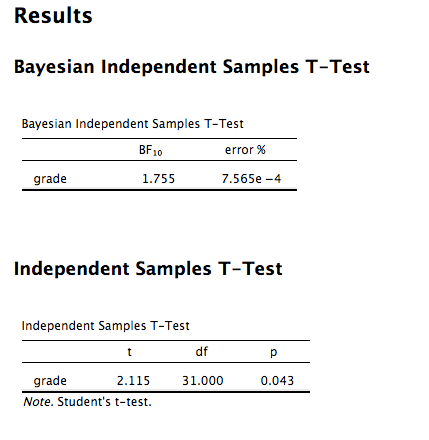
\epsfig{file = ../img/bayes/bayes1.png,clip=true, width = 10cm} 
\caption{Bayesian independent Samples $t$-test result in JASP}
\label{fig:bayes1}
\HR
\end{center}
\end{figure}

What does the Bayesian version of the $t$-test look like? We can get the Bayes factor analysis by selecting the `T-Tests' - `Bayesian Independent Samples T-Test' option.  The dialog is similar to the conventional $t$-test from earlier, so you should already know what to do!  For now, just accept the defaults that JASP provides. This gives the results shown in the table in Figure \ref{fig:bayes1}. What we get in this table is a Bayes factor statistic of 1.755, meaning that the evidence provided by these data are about 1.8:1 in favour of the alternative hypothesis. 

Before moving on, it's worth highlighting the difference between the orthodox test results and the Bayesian one. According to the orthodox test, we obtained a significant result, though only barely. Nevertheless, many people would happily accept $p=.043$ as reasonably strong evidence for an effect. In contrast, notice that the Bayesian test doesn't even reach 2:1 odds in favour of an effect, and would be considered very weak evidence at best. In my experience that's a pretty typical outcome. Bayesian methods usually require more evidence before rejecting the null.

\SUBSECTION{Paired samples \texorpdfstring{$t$}{t}-test}

Back in Section~\ref{sec:pairedsamplesttest} I discussed the \rtext{chico.csv} data set in which student grades were measured on two tests, and we were interested in finding out whether grades went up from test 1 to test 2. Because every student did both tests, the tool we used to analyse the data was a paired samples $t$-test. Figure \ref{fig:bayes3} shows the JASP results table for the conventional paired $t$-test alongside the Bayes factor analysis. At this point, I hope you can read this output without any difficulty. The data provide evidence of about 6000:1 in favour of the alternative. We could probably reject the null with some confidence!

\begin{figure}[ht]
\begin{center}
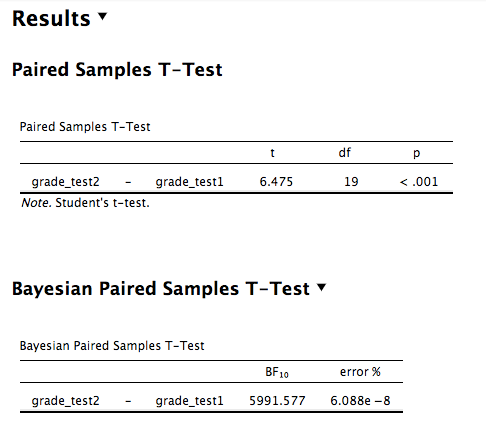
\epsfig{file = ../img/bayes/bayes3.png,clip=true, width = 10cm} 
\caption{Paired samples T-Test and Bayes Factor result in JASP}
\label{fig:bayes3}
\HR
\end{center}
\end{figure}


\begin{comment}
\section{Bayesian regression~\label{sec:bayesregression}}

Okay, so now we've seen Bayesian equivalents to orthodox chi-square tests and $t$-tests. What's next? If I were to follow the same progression that I used when developing the orthodox tests you'd expect to see ANOVA next, but I think it's a little clearer if we start with regression. 

\SUBSECTION{A quick refresher}

In Chapter~\ref{ch:regression} I used the \rtext{parenthood} data to illustrate the basic ideas behind regression. To remind you of what that data set looks like, here's the first six observations:
\begin{rblock1}
> @usr{load("parenthood.Rdata")}
> @usr{head(parenthood)}
  dan.sleep baby.sleep dan.grump day
1      7.59      10.18        56   1
2      7.91      11.66        60   2
3      5.14       7.92        82   3
4      7.71       9.61        55   4
5      6.68       9.75        67   5
6      5.99       5.04        72   6
\end{rblock1}

\noindent
Back in Chapter~\ref{ch:regression} I proposed a theory in which my grumpiness (\rtext{dan.grump}) on any given day is related to the amount of sleep I got the night before (\rtext{dan.sleep}), and possibly to the amount of sleep our baby got (\rtext{baby.sleep}), though probably not to the \rtext{day} on which we took the measurement. We tested this using a regression model. In order to estimate the regression model we used the \rtext{lm()} function, like so:

\begin{rblock1}
> @usr{model <- lm(} 
+ @usr{   formula = dan.grump ~ dan.sleep + day + baby.sleep,}
+ @usr{   data = parenthood}
+ @usr{)}
\end{rblock1}
The hypothesis tests for each of the terms in the regression model were extracted using the \rtext{summary()} function, a (somewhat truncated) version of which is shown below:
\begin{rblock1}
> @usr{summary(model)}

BLAH BLAH BLAH

Coefficients:
              Estimate Std. Error t value Pr(>|t|)    
(Intercept) 126.278707   3.242492  38.945   <2e-16 ***
dan.sleep    -8.969319   0.560007 -16.016   <2e-16 ***
day          -0.004403   0.015262  -0.288    0.774    
baby.sleep    0.015747   0.272955   0.058    0.954    

BLAH BLAH BLAH
\end{rblock1}
When interpreting the results, each row in this table corresponds to one of the possible predictors. The \rtext{(Intercept)} term isn't usually interesting, though it is highly significant. The important thing for our purposes is the fact that \rtext{dan.sleep} is significant at $p<.001$ and neither of the other variables are. 

\subsection{The Bayesian version}

Okay, so how do we do the same thing using the \rtext{BayesFactor} package? The easiest way is to use the \rtext{regressionBF()} function instead of \rtext{lm()}. As before, we use \rtext{formula} to indicate what the full regression model looks like, and the \rtext{data} argument to specify the data frame. So the command is:

\begin{rblock1}
> @usr{regressionBF(}
+ @usr{   formula = dan.grump ~ dan.sleep + day + baby.sleep,}
+ @usr{   data = parenthood}
+ @usr{)}
\end{rblock1}

\noindent
So that's pretty straightforward: it's exactly what we've been doing throughout the book. The output, however, is a little different from what you get from \rtext{lm()}. Here's what we get:

\begin{rblock1}
Bayes factor analysis
--------------
[1] dan.sleep                    : 1.622545e+34 @plusorminus0%
[2] day                          : 0.2724027    @plusorminus0%
[3] baby.sleep                   : 10018411     @plusorminus0%
[4] dan.sleep + day              : 1.016578e+33 @plusorminus0.01%
[5] dan.sleep + baby.sleep       : 9.770233e+32 @plusorminus0.01%
[6] day + baby.sleep             : 2340755      @plusorminus0%
[7] dan.sleep + day + baby.sleep : 7.835625e+31 @plusorminus0%

Against denominator:
  Intercept only 
---
Bayes factor type: BFlinearModel, JZS
\end{rblock1}
The format of this is pretty familiar. At the bottom we have some techical rubbish, and at the top we have some information about the Bayes factors. What's new is the fact that we seem to have {\it lots} of Bayes factors here. What's all this about?

The trick to understanding this output is to recognise that if we're interested in working out which of the 3 predictor variables are related to \rtext{dan.grump}, there are actually 8 possible regression models that could be considered. One possibility is the {\it intercept only model}, in which none of the three variables have an effect. At the other end of the spectrum is the {\it full model} in which all three variables matter. So what \rtext{regressionBF()} does is treat the {\it intercept only} model as the null hypothesis, and print out the Bayes factors for all other models when compared against that null. For example, if we look at line 4 in the table, we see that the evidence is about $10^{33}$ to 1 in favour of the claim that a model that includes both \rtext{dan.sleep} and \rtext{day} is better than the intercept only model. Or if we look at line 1, we can see that the odds are about $1.6 \times 10^{34}$ that a model containing the \rtext{dan.sleep} variable (but no others) is better than the intercept only model.


\SUBSECTION{Finding the best model}

In practice, this isn't super helpful. In most situations the intercept only model is one that you don't really care about at all. What I find helpful is to start out by working out which model is the {\it best} one, and then seeing how well all the alternatives compare to it. Here's how you do that. In this case, it's easy enough to see that the best model is actually the one that contains \rtext{dan.sleep} only (line 1), because it has the largest Bayes factor. However, if you've got a lot of possible models in the output, it's handy to know that you can use the \rtext{head()} function to pick out the best few models. First, we have to go back and save the Bayes factor information to a variable:

\begin{rblock1}
> @usr{models <- regressionBF(}
+ @usr{   formula = dan.grump ~ dan.sleep + day + baby.sleep,}
+ @usr{   data = parenthood}
+ @usr{)}
\end{rblock1}

\noindent
Let's say I want to see the best three models. To do this, I use the \rtext{head()} function specifying \rtext{n=3}, and here's what I get as the result:
\begin{rblock1}
> @usr{head( models, n = 3)}

Bayes factor analysis
--------------
[1] dan.sleep              : 1.622545e+34 @plusorminus0%
[2] dan.sleep + day        : 1.016578e+33 @plusorminus0.01%
[3] dan.sleep + baby.sleep : 9.770233e+32 @plusorminus0.01%

Against denominator:
  Intercept only 
---
Bayes factor type: BFlinearModel, JZS
\end{rblock1}
This is telling us that the model in line 1 (i.e., \rtextverb#dan.grump ~ dan.sleep#) is the best one. That's {\it almost} what I'm looking for, but it's still comparing all the models against the intercept only model. That seems silly. What I'd like to know is how big the difference is between the best model and the other good models. For that, there's this trick:



\begin{rblock1}
> @usr{head( models/max(models), n = 3)}

Bayes factor analysis
--------------
[1] dan.sleep              : 1          @plusorminus0%
[2] dan.sleep + day        : 0.06265328 @plusorminus0.01%
[3] dan.sleep + baby.sleep : 0.06021549 @plusorminus0.01%

Against denominator:
  dan.grump ~ dan.sleep 
---
Bayes factor type: BFlinearModel, JZS
\end{rblock1}
Notice the bit at the bottom showing that the ``denominator'' has changed. What that means is that the Bayes factors are now comparing each of those 3 models listed against the \rtextverb#dan.grump ~ dan.sleep# model. Obviously, the Bayes factor in the first line is exactly 1, since that's just comparing the best model to itself. More to the point, the other two Bayes factors are both less than 1, indicating that they're all worse than that model. The Bayes factors of 0.06 to 1 imply that the odds for the best model over the second best model are about 16:1. You can work this out by simple arithmetic (i.e., $0.06 / 1 \approx 16$), but the other way to do it is to directly compare the models. To see what I mean, here's the original output:

\begin{rblock1}
> @usr{models}
Bayes factor analysis
--------------
[1] dan.sleep                    : 1.622545e+34 @plusorminus0%
[2] day                          : 0.2724027    @plusorminus0%
[3] baby.sleep                   : 10018411     @plusorminus0%
[4] dan.sleep + day              : 1.016578e+33 @plusorminus0.01%
[5] dan.sleep + baby.sleep       : 9.770233e+32 @plusorminus0.01%
[6] day + baby.sleep             : 2340755      @plusorminus0%
[7] dan.sleep + day + baby.sleep : 7.835625e+31 @plusorminus0%

Against denominator:
  Intercept only 
---
Bayes factor type: BFlinearModel, JZS
\end{rblock1}
The best model corresponds to row 1 in this table, and the second best model corresponds to row 4. All you have to do to compare these two models is this:

\begin{rblock1}
> @usr{models[1] / models[4]}

Bayes factor analysis
--------------
[1] dan.sleep : 15.96086 @plusorminus0.01%

Against denominator:
  dan.grump ~ dan.sleep + day 
---
Bayes factor type: BFlinearModel, JZS
\end{rblock1}
And there you have it. You've found the regression model with the highest Bayes factor (i.e., \rtextverb#dan.grump ~ dan.sleep#), and you know that the evidence for that model over the next best alternative (i.e., \rtextverb#dan.grump ~ dan.sleep + day#) is about 16:1.


\SUBSECTION{Extracting Bayes factors for all included terms}

Okay, let's say you've settled on a specific regression model. What Bayes factors should you report? In this example, I'm going to pretend that you decided that \rtextverb#dan.grump ~ dan.sleep + baby.sleep# is the model you think is best. Sometimes it's sensible to do this, even when it's not the one with the highest Bayes factor. Usually this happens because you have a substantive theoretical reason to prefer one model over the other. However, in this case I'm doing it because I want to use a model with more than one predictor as my example! 

Having figured out which model you prefer, it can be really useful to call the \rtext{regressionBF()} function and specifying  \rtext{whichModels="top"}. You use your ``preferred'' model as the \rtext{formula} argument, and then the output will show you the Bayes factors that result when you try to drop predictors from this model:
\begin{rblock1}
> @usr{regressionBF( }
+ @usr{  formula = dan.grump ~ dan.sleep + baby.sleep,}
+ @usr{  data = parenthood,}
+ @usr{  whichModels = "top"}
+ @usr{)}

Bayes factor top-down analysis
--------------
When effect is omitted from dan.sleep + baby.sleep , BF is...
[1] Omit baby.sleep : 16.60702     @plusorminus0.01%
[2] Omit dan.sleep  : 1.025401e-26 @plusorminus0.01%

Against denominator:
  dan.grump ~ dan.sleep + baby.sleep 
---
Bayes factor type: BFlinearModel, JZS
\end{rblock1}
Okay, so now you can see the results a bit more clearly. The Bayes factor when you try to drop the \rtext{dan.sleep} predictor is about $10^{-26}$, which is very strong evidence that you {\it shouldn't} drop it. On the other hand, the Bayes factor actually goes up to 17 if you drop \rtext{baby.sleep}, so you'd usually say that's pretty strong evidence for dropping that one.

\section{Bayesian ANOVA~\label{sec:bayesanova}}

As you can tell, the \rtext{BayesFactor} package is pretty flexible, and it can do Bayesian versions of pretty much everything in this book. In fact, it can do a few other neat things that I haven't covered in the book at all. However, I have to stop somewhere, and so there's only one other topic I want to cover: Bayesian ANOVA. 

\SUBSECTION{A quick refresher}

As with the other examples, I think it's useful to start with a reminder of how I discussed ANOVA earlier in the book. First, let's remind ourselves of what the data were. The example I used originally is the \rtext{clin.trial} data frame, which looks like this

\begin{rblock1}
> @usr{load("clinicaltrial.Rdata")}
> @usr{head(clin.trial)}
      drug    therapy mood.gain
1  placebo no.therapy       0.5
2  placebo no.therapy       0.3
3  placebo no.therapy       0.1
4 anxifree no.therapy       0.6
5 anxifree no.therapy       0.4
6 anxifree no.therapy       0.2
\end{rblock1}

\noindent
To run our orthodox analysis in earlier chapters we used the \rtext{aov()} function to do all the heavy lifting. In Chapter~\ref{ch:anova2} I recommended using the \rtext{Anova()} function from the \rtext{car} package to produce the ANOVA table, because it uses Type II tests by default. If you've forgotten what ``Type II tests'' are, it might be a good idea to re-read Section~\ref{sec:unbalancedanova}, because it will become relevant again in a moment. In any case, here's what our analysis looked like:
\begin{rblock1}
> @usr{model <- aov( mood.gain ~ drug * therapy, data = clin.trial )}
> @usr{Anova(model)}
Anova Table (Type II tests)

Response: mood.gain
             Sum Sq Df F value    Pr(>F)    
drug         3.4533  2 31.7143 1.621e-05 ***
therapy      0.4672  1  8.5816   0.01262 *  
drug:therapy 0.2711  2  2.4898   0.12460             
\end{rblock1}
That's pretty clearly showing us evidence for a main effect of \rtext{drug} at $p<.001$, an effect of \rtext{therapy} at $p<.05$ and no interaction. 

\SUBSECTION{The Bayesian version}

How do we do the same thing using Bayesian methods? The \rtext{BayesFactor} package contains a function called \rtext{anovaBF()} that does this for you. It uses a pretty standard \rtext{formula} and \rtext{data} structure, so the command should look really familiar. Just like we did with regression, it will be useful to save the output to a variable:
\begin{rblock1}
> @usr{models <- anovaBF( }
+ @usr{  formula = mood.gain ~ drug * therapy,}
+ @usr{  data = clin.trial}
+ @usr{)}
\end{rblock1}

\noindent
The output is quite different to the traditional ANOVA, but it's not too bad once you understand what you're looking for. Let's take a look:
\begin{rblock1}
> @usr{models}

Bayes factor analysis
--------------
[1] drug                          : 245.9026  @plusorminus0%
[2] therapy                       : 0.7316007 @plusorminus0%
[3] drug + therapy                : 698.3343  @plusorminus0.96%
[4] drug + therapy + drug:therapy : 688.3077  @plusorminus1.3%

Against denominator:
  Intercept only 
---
Bayes factor type: BFlinearModel, JZS
\end{rblock1}

\noindent
This looks very similar to the output we obtained from the \rtext{regressionBF()} function, and with good reason. Remember what I said back in Section~\ref{sec:anovalm}: under the hood, ANOVA is no different to regression, and both are just different examples of a linear model. Becasue of this, the  \rtext{anovaBF()} reports the output in much the same way. For instance, if we want to identify the best model we could use the same commands that we used in the last section. One variant that I find quite useful is this:

\begin{rblock1}
> @usr{models/max(models)}

Bayes factor analysis
--------------
[1] drug                          : 0.3521273   @plusorminus0.96%
[2] therapy                       : 0.001047637 @plusorminus0.96%
[3] drug + therapy                : 1           @plusorminus0%
[4] drug + therapy + drug:therapy : 0.9856421   @plusorminus1.62%

Against denominator:
  mood.gain ~ drug + therapy 
---
Bayes factor type: BFlinearModel, JZS
\end{rblock1}
By ``dividing'' the \rtext{models} output by the best model (i.e., \rtext{max(models)}), what \R\ is doing is using the best model (which in this case is \rtext{drugs + therapy}) as the denominator, which gives you a pretty good sense of how close the competitors are. For instance, the model that contains the interaction term is almost as good as the model without the interaction, since the Bayes factor is 0.98. In other words, the data do not clearly indicate whether there is or is not an interaction.  

\SUBSECTION{Constructing Bayesian Type II tests}

Okay, that's all well and good, you might be thinking, but what do I report as the alternative to the $p$-value? In the classical ANOVA table, you get a single $p$-value for every predictor in the model, so you can talk about the significance of each effect. What's the Bayesian analog of this?

It's a good question, but the answer is tricky. Remember what I said in Section~\ref{sec:unbalancedanova} about ANOVA being complicated. Even in the classical version of ANOVA there are several different ``things'' that ANOVA might correspond to. Specifically, I discussed how you get different $p$-values depending on whether you use Type I tests, Type II tests or Type III tests. To work out which Bayes factor is analogous to ``the'' $p$-value in a classical ANOVA, you need to work out which version of ANOVA you want an analog for. For the purposes of this section, I'll assume you want Type II tests, because those are the ones I think are most sensible in general. As I discussed back in Section~\ref{sec:unbalancedanova}, Type II tests for a two-way ANOVA are reasonably straightforward, but if you have forgotten that section it wouldn't be a bad idea to read it again before continuing.

Assuming you've had a refresher on Type II tests, let's have a look at how to pull them from the Bayes factor table. Suppose we want to test the main effect of \rtext{drug}. The null hypothesis for this test corresponds to a model that includes an effect of \rtext{therapy}, but no effect of \rtext{drug}. The alternative hypothesis is the model that includes both. In other words, what we want is the Bayes factor corresponding to this comparison:

\vspace*{3pt}\hspace*{2cm}\begin{tabular}{ll}
Null model: & \rtextverb#mood.gain ~ therapy# \\
Alternative model: & \rtextverb#mood.gain ~ therapy + drug#
\end{tabular}\vspace*{3pt}

\noindent
As it happens, we can read the answer to this straight off the table because it corresponds to a comparison between the model in line 2 of the table and the model in line 3: the Bayes factor in this case  represents evidence {\it for} the null of 0.001 to 1. Or, more helpfully, the odds are about 1000 to 1 against the null. 

The main effect of \rtext{therapy} can be calculated in much the same way. In this case, the null model is the one that contains only an effect of drug, and the alternative is the model that contains both. So the relevant comparison is between lines 2 and 1 in the table. The odds in favour of the null here are only 0.35 to 1. Again, I find it useful to frame things the other way around, so I'd refer to this as evidence of about 3 to 1 in favour of an effect of \rtext{therapy}.

Finally, in order to test an interaction effect, the null model here is one that contains both main effects but no interaction. The alternative model adds the interaction. That is:

\vspace*{3pt}\hspace*{2cm}\begin{tabular}{ll}
Null model: & \rtextverb#mood.gain ~ drug + therapy# \\
Alternative model: & \rtextverb#mood.gain ~ drug + therapy + drug:therapy#
\end{tabular}\vspace*{3pt}

\noindent
If we look those two models up in the table, we see that this comparison is between the models on lines 3 and 4 of the table. The odds of 0.98 to 1 imply that these two models are fairly evenly matched.

You might be thinking that this is all pretty laborious, and I'll concede that's true. At some stage I might consider adding a function to the \rtext{lsr} package that would automate this process and construct something like a ``Bayesian Type II ANOVA table'' from the output of the \rtext{anovaBF()} function. However, I haven't had time to do this yet, nor have I made up my mind about whether it's really a good idea to do this. In the meantime, I thought I should show you the trick for how I do this in practice. The command that I use when I want to grab the right Bayes factors for a Type II ANOVA is this one:

\begin{rblock1}
> @usr{max(models)/models}

                denominator
numerator            drug  therapy drug + therapy drug + therapy + drug:therapy
  drug + therapy 2.839882 954.5292              1                      1.014567 
\end{rblock1}

\noindent
The output isn't quite so pretty as the last one, but the nice thing is that you can read off everything you need. The best model is \rtext{drug + therapy}, so all the other models are being compared to that. What's the Bayes factor {\it for} the main effect of \rtext{drug}? The relevant null hypothesis is the one that contains only \rtext{therapy}, and the Bayes factor in question is 954:1. The main effect of \rtext{therapy} is weaker, and the evidence here is only 2.8:1. Finally, the evidence {\it against} an interaction is very weak, at 1.01:1.

Reading the results off this table is sort of counterintuitive, because you have to read off the answers from the ``wrong'' part of the table. For instance, the evidence for an effect of \rtext{drug} can be read from the column labelled \rtext{therapy}, which is pretty damned weird. To be fair to the authors of the package, I don't think they ever intended for the \rtext{anovaBF()} function to be used this way. My understanding\FOOTNOTE{Again, guys, sorry if I've misread you.} is that their view is simply that you should find the best model and report that model: there's no inherent reason why a Bayesian ANOVA should try to follow the exact same design as an orthodox ANOVA.\FOOTNOTE{I don't even disagree with them: it's {\it not} at all obvious why a Bayesian ANOVA should reproduce (say) the same set of model comparisons that the Type II testing strategy uses. It's precisely because of the fact that I haven't really come to any strong conclusions that I haven't added anything to the \rtext{lsr} package to make Bayesian Type II tests easier to produce.}

In any case, if you know what you're looking for, you can look at this table and then report the results of the Bayesian analysis in a way that is pretty closely analogous to how you'd report a regular Type II ANOVA. As I mentioned earlier, there's still no convention on how to do that, but I usually go for something like this:

\begin{quote}
A Bayesian Type II ANOVA found evidence for main effects of drug (Bayes factor: 954:1) and therapy (Bayes factor: 3:1), but no clear evidence for or against an interaction (Bayes factor: 1:1). 
\end{quote}



\end{comment}


\section{Summary}

The first half of this chapter was focused primarily on the theoretical underpinnings of Bayesian statistics. I introduced the mathematics for how Bayesian inference works (Section~\ref{sec:basicbayes}), and gave a very basic overview of how Bayesian hypothesis testing is typically done (Section~\ref{sec:bayesianhypothesistests}). Finally, I devoted some space to talking about why I think Bayesian methods are worth using (Section \ref{sec:whybayes}).

Then I gave a practical example, a Bayesian $t$-test (Section~\ref{sec:ttestbf}). If you're interested in learning more about the Bayesian approach, there are many good books you could look into. John Kruschke's book {\it Doing Bayesian Data Analysis} is a pretty good place to start \parencite{Kruschke2011} and is a nice mix of theory and practice. His approach is a little different to the ``Bayes factor'' approach that I've discussed here, so you won't be covering the same ground. If you're a cognitive psychologist, you might want to check out Michael Lee and E.J. Wagenmakers' book {\it Bayesian Cognitive Modeling} \parencite{Lee2014}. I picked these two because I think they're especially useful for people in my discipline, but there's a lot of good books out there, so look around!




